% ==============================================================================
% Beamer Presentation Template
% ------------------------------------------------------------------------------
% Non-official presentation template made by Heitor Gama.
%
% This file is intended as a reusable starting point for technical presentations.
% Replace the metadata, examples, figures, and references for each new talk.
% Keep the layout commands together so future presentations can be edited from
% this file.
% ==============================================================================

\documentclass[aspectratio=169]{beamer}
\usepackage[utf8]{inputenc}
\usepackage[T1]{fontenc}
\usepackage{amsmath}
\usepackage{graphicx}
\usepackage[table]{xcolor}
\usepackage{multirow}
\usepackage{hhline}
\usepackage{booktabs}
\usepackage{caption}
\usepackage{tabularx,array}
\usepackage{tikz}
\usetikzlibrary{calc}
\usepackage{hyperref}
\usepackage{biblatex}

\addbibresource{references.bib}
\setbeamerfont{footnote}{size=\tiny}
\renewcommand{\cite}[1]{\texorpdfstring{\footfullcite{#1}}{}}
\newcommand{\todo}[1]{{\color{red} TODO: #1}}

% Redefine table and figure captions to include numbering.
\setbeamertemplate{caption}[numbered]
\renewcommand{\thetable}{\arabic{table}}
\renewcommand{\thefigure}{\arabic{figure}}
\setbeamertemplate{caption label}{\insertcaptionname~\insertcaptionnumber}

%====================== TEMPLATE METADATA ======================

\title[Technical Presentation Title]{{\bf \Huge Technical Presentation Template}}
\author[Heitor Gama]{\texorpdfstring{\textbf{Heitor Gama}\\Escola Polit\'ecnica da USP}{Heitor Gama, Escola Politecnica da USP}}
\date{}

\newcommand{\presentationcontext}{Course, project, seminar, supervisors or conference track}
\newcommand{\presenteremail}{heitor\_gama@usp.br}
\newcommand{\presenterwebsite}{https://www.heitor-gama.com}

%====================== THEME AND LAYOUT ======================

\setbeamertemplate{navigation symbols}{}
\setbeamertemplate{footline}{}
\setbeamertemplate{itemize item}[circle]
\setbeamertemplate{itemize subitem}[circle]
\setbeamertemplate{itemize subsubitem}[circle]

\setbeamercolor{title}{fg=black}
\setbeamercolor{frametitle}{fg=black}
\setbeamercolor{structure}{fg=black}
\setbeamercolor{item}{fg=black}

\makeatletter
\setbeamertemplate{sidebar right}{%
  \ifnum\c@framenumber>1
    \vbox to \paperheight{%
      \vspace*{0.35em}%
      \hbox{%
        \hspace*{-2.62em}%
        \rotatebox{270}{%
          \colorbox{black}{%
            \textcolor{white}{\scriptsize SLIDE \insertframenumber}%
          }%
        }%
      }%
      \vfill
    }%
  \fi
}
\makeatother

\usebackgroundtemplate{%
  
\includegraphics[width=\paperwidth,height=\paperheight]{figures/background.png}%
}

\newcommand{\mysubtitle}[1]{%
  \vspace{-0.3em}
  {\small\textit{\textcolor[rgb]{0.49,0.49,0.49}{#1}}}
}

\setbeamertemplate{frametitle}{%
  \vspace{0.5em}
  \textbf{\insertframetitle}\\
  \vspace{0.1em}
  \mysubtitle{\insertframesubtitle}
  \hfill
  \vspace{0.3em}
  \hrule height 0.2pt
  \begin{tikzpicture}[remember picture,overlay]
    \node[anchor=north east, yshift=0em, xshift=-2em] at (current page.north east) {
      
\includegraphics[height=2.5em]{figures/crossing_small.pdf}
    };
  \end{tikzpicture}
}

\newcommand{\fixedtopspacing}{\vspace{0.35em}}

\newcommand{\websiteicon}{%
  \raisebox{\dimexpr0.5ex-0.5\height\relax}{%
    \tikz[x=0.08em,y=0.08em,line width=0.07em]{
      \draw (0,0) circle (5);
      \draw (-5,0) -- (5,0);
      \draw (0,-5) arc[start angle=-90,end angle=90,x radius=2.3,y radius=5];
      \draw (0,-5) arc[start angle=-90,end angle=-270,x radius=2.3,y radius=5];
    }%
  }%
}

\newcommand{\mailicon}{%
  \raisebox{\dimexpr0.5ex-0.5\height\relax}{%
    \tikz[x=0.09em,y=0.09em,line width=0.07em]{
      \draw (-5,-3) rectangle (5,3);
      \draw (-5,3) -- (0,-0.6) -- (5,3);
      \draw (-5,-3) -- (-1,-0.4);
      \draw (5,-3) -- (1,-0.4);
    }%
  }%
}

\newsavebox{\circlephotobox}
\newcommand{\circlephoto}[2]{%
  \sbox{\circlephotobox}{\includegraphics{#1}}%
  \begin{tikzpicture}
    \path[use as bounding box] (-#2,-#2) rectangle (#2,#2);
    \begin{scope}
      \clip (0,0) circle[radius=#2];
      \ifdim\wd\circlephotobox>\ht\circlephotobox
        \node[inner sep=0pt] at (0,0) {\includegraphics[height=\dimexpr#2+#2\relax]{#1}};
      \else
        \node[inner sep=0pt] at (0,0) {\includegraphics[width=\dimexpr#2+#2\relax]{#1}};
      \fi
    \end{scope}
  \end{tikzpicture}%
}

\newcommand{\checkedbox}{%
  \raisebox{\dimexpr0.5ex-0.5\height\relax}{%
    \tikz[x=0.95em,y=0.95em,line width=0.055em]{
      \draw (0,0) rectangle (0.85,0.85);
      \draw (0.18,0.43) -- (0.36,0.22) -- (0.7,0.65);
    }%
  }%
}

\newcommand{\checklistitem}[1]{%
  \par\noindent\checkedbox\hspace{0.5em}%
  \begin{minipage}[t]{0.88\linewidth}#1\end{minipage}\par\vspace{0.45em}%
}

\newcommand{\circledvalue}[1]{%
  \makebox[0pt][l]{%
    \raisebox{-0.15ex}{%
      \tikz[remember picture,overlay]{
        \draw[red,line width=0.7pt] (1.1,0.14) ellipse [x radius=1.4cm,y radius=0.28cm];
      }%
    }%
  }#1%
}

\newcommand{\sectionframe}[1]{%
  \begin{frame}{}
    \vfill
    \begin{center}
      \Huge \textbf{#1}
    \end{center}
    \vfill
  \end{frame}
}

%====================== DOCUMENT ======================

\begin{document}

\begin{frame}[plain]
  \titlepage
  \vspace{-1.7cm}
  \centering
  {\large \presentationcontext}\\[0.7cm]
  
\includegraphics[height=3em]{figures/Crossing_logo_name_BonW.pdf}
\end{frame}

\begin{frame}{About me}{Heitor Gama}
\fixedtopspacing
\begin{columns}[T,onlytextwidth]
  \begin{column}{0.35\textwidth}
    \centering
    \circlephoto{figures/heitor.jpg}{1.8cm}\\[0.35em]
    \resizebox{\linewidth}{!}{\websiteicon\hspace{0.35em}\href{\presenterwebsite}{\presenterwebsite}}
  \end{column}
  \begin{column}{0.64\textwidth}
    \small
    \begin{itemize}
      \item Computer Engineering student at Escola Polit\'ecnica da USP, double degree at CentraleSup\'elec.
      \item Research on Explainable AI at MICS, CentraleSup\'elec.
      \item Previous research with IRL CNRS Crossing on LLMs for multi-agent search-and-rescue settings.
      \item Interests include explainable AI, reinforcement learning, computer vision, technical competitions, and applied AI systems.
      \item Research experience across Brazil, France, and Australia.
    \end{itemize}
  \end{column}
\end{columns}
\end{frame}

\sectionframe{Introduction}

\begin{frame}{Start from the audience}{One message per slide}
\fixedtopspacing
\begin{itemize}
  \item A slide is not a paper page. It should only support what the speaker says instead of replacing it.
  \item State the slide's purpose in the title or subtitle before adding visual detail.
  \item Prefer one central claim, comparison, diagram, table, or equation per slide.
  \item Reveal content step by step if the order helps the explanation.
  \item Move dense derivations, long code, and exhaustive tables to backup slides.
\end{itemize}
\end{frame}

\begin{frame}{Use the title and subtitle deliberately}{Make the frame readable before the content}
\fixedtopspacing
\begin{itemize}
  \item Use the title for the object of discussion, such as a method, result, limitation, or question.
  \item Subtitles are optional. I like to use them for the interpretation, the slide takeaway.
  \item If the slide needs a long explanation to be understood, split it.
\end{itemize}
\end{frame}

\sectionframe{Related Work}

\begin{frame}{Structure the talk}{Separate navigation from content}
\fixedtopspacing
\begin{table}[h]
\centering
\small
\begin{tabularx}{0.92\textwidth}{lX}
\toprule
\textbf{Part} & \textbf{What it should do} \\
\midrule
Opening & Establish the topic, speaker, affiliation, and talk context. \\
Motivation & Explain the problem and why the audience should care now. \\
Method & Show the bare minimum needed to understand the result. \\
Evidence & Present figures, tables, comparisons, or case studies. \\
Close & Summarize the contribution, limits, next steps, and contact path. \\
\bottomrule
\end{tabularx}
\caption{A reusable talk structure. You might want to present your specific section summary at the start of the talk if the presentation is long.}
\end{table}
\end{frame}

\begin{frame}{Cite close to the claim}{Footnote citations work well in talks}
\fixedtopspacing
\begin{itemize}
  \item Put citations near the exact claim they support.
  \item Use a footnote citation when the audience should see the source without interrupting the slide.\cite{li2023theory}
  \item Cite baselines, benchmarks, and reused methods when they shape your comparison.\cite{yu2022surprising}
  \item Keep the references slide for checking details after the talk.
  \item Use a single bibliography style across all entries.
\end{itemize}
\end{frame}

\sectionframe{Methods}

\begin{frame}{Prefer vector figures}{Use raster formats only when the data is raster}
\fixedtopspacing
\begin{columns}[T,onlytextwidth]
  \begin{column}{0.5\textwidth}
    \begin{figure}
      \centering
      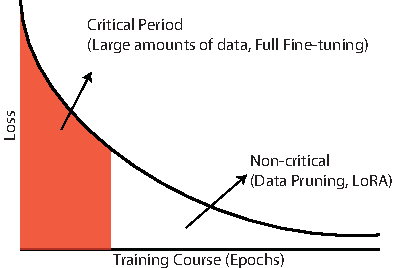
\includegraphics[width=0.9\linewidth,keepaspectratio]{figures/teaser.pdf}
      \caption{Vector diagrams and plots stay sharp when projected or exported.}
    \end{figure}
  \end{column}
  \begin{column}{0.5\textwidth}
    \small
    \begin{itemize}
      \item Images should be the clearest possible, even when projected on a large screen, low quality projectors or viewed from the back of a room.
      \item Use PDF for diagrams, plots, graphs, and schematic figures. In matplotlib, for example, it is very simple to save figures as PDF.
      \item Rebuild from scratch your diagrams in a vector format.
      \item PNG/JPEG allowed only for pixel-level image data or actual photos!
    \end{itemize}
  \end{column}
\end{columns}
\end{frame}

\begin{frame}{Keep equations compact}{Define symbols immediately}
\fixedtopspacing
\begin{itemize}
  \item Show only the equation needed for the argument.
  \item Define every symbol before or immediately after the equation.
\end{itemize}
\vspace{0.5cm}
\begin{equation}
  S = \frac{1}{n}\sum_{i=1}^{n} w_i x_i,
\end{equation}
where \(S\) is the summary score, \(x_i\) is one observed component, and \(w_i\) is its weight.
\end{frame}

\sectionframe{Results}

\begin{frame}{Make tables earn their space}{Show relevant comparisons}
\fixedtopspacing
\vspace{0.55cm}
\begin{table}[h]
\centering
\small
\begin{tabular}{lccc}
\toprule
\textbf{Version} & \textbf{Text density} & \textbf{Visual anchor} & \textbf{Audience task} \\
\midrule
Draft & High & None & Decode everything live \\
Readable & Medium & Highlighted row & Compare key cases \\
Talk-ready & Low & Claim + contrast & Remember the takeaway \\
\bottomrule
\end{tabular}
\caption{Use tables when precise comparison is the point. Highlight rows or columns discussed out loud.}
\end{table}
\end{frame}

\begin{frame}{Highlight the table before interpreting it}{Use color or circles to direct attention}
\fixedtopspacing
\vspace{0.35cm}
\begin{table}[h]
\centering
\scalebox{0.82}{
\begin{tabular}{l l c c c}
\toprule
\textbf{Agents} & \textbf{Map (\#Nodes)} & \textbf{Score} & \textbf{Rounds to Completion} & \textbf{Valid Action \%} \\
\midrule
o4-mini & Default (5)  & $90 \pm 0.00$      & $13 \pm 3.00$   & 95.83\% \\
o4-mini & Medium (8)   & $90 \pm 0.00$      & $14 \pm 3.46$   & 97.22\% \\
o4-mini & Hard (16)    & $90 \pm 0.00$      & $20 \pm 3.46$   & 98.80\% \\
\only<1-2>{o4-mini}\only<3->{\cellcolor{red!18}o4-mini} &
\only<1-2>{Village (53)}\only<3->{\cellcolor{red!18}Village (53)} &
\only<1>{$83.33 \pm 11.55$}\only<2>{\circledvalue{$83.33 \pm 11.55$}}\only<3->{\cellcolor{red!18}$83.33 \pm 11.55$} &
\only<1-2>{$79.33 \pm 28.22$}\only<3->{\cellcolor{red!18}$79.33 \pm 28.22$} &
\only<1-2>{95.25\%}\only<3->{\cellcolor{red!18}95.25\%} \\
\bottomrule
\end{tabular}}
\caption{The complete table. Then one value circled. Then one row highlighted.}
\end{table}
\only<2>{\vspace{0.2cm}\centering\small A circle is useful when only one number needs attention.\par}
\only<3->{\vspace{0.2cm}\centering\small A row highlight is useful when the full case is being discussed.\par}
\end{frame}

\begin{frame}{Label visuals where readers look}{Reduce caption dependency}
\fixedtopspacing
\begin{columns}[T,onlytextwidth]
  \small
  \begin{column}{0.7\textwidth}
    \begin{figure}
      \vspace{-0.5cm}
      \centering
      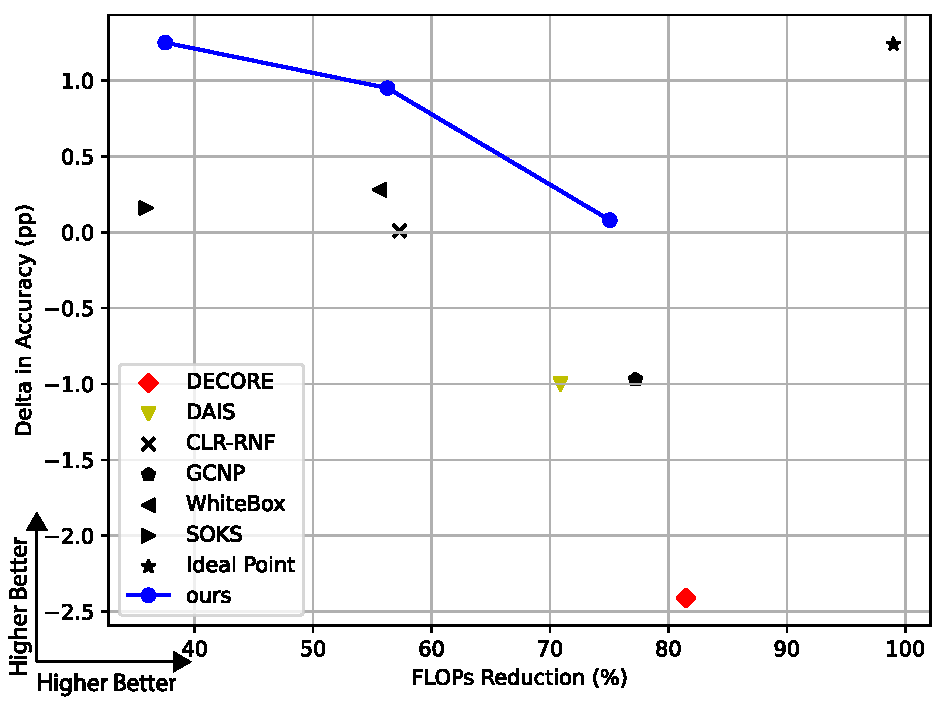
\includegraphics[width=0.7\linewidth,keepaspectratio]{figures/sample_figure.pdf}
      \caption{\small Different shape patterns help readers distinguish between groups and brings colorblind accessibility.}
    \end{figure}
  \end{column}
  \hspace{-0.2\textwidth}
  \begin{column}{0.37\textwidth}
    \begin{itemize}
      \item Captions are still useful, but the visual should not depend on them completely.
      \item Put labels and units in axis.
      \item Avoid plot titles that repeat the slide title.
      \item Use color plus shape, texture, line style, or text labels.
    \end{itemize}
  \end{column}
\end{columns}
\end{frame}

\sectionframe{Discussion}

\begin{frame}{Use backup slides}{Keep the main story uncluttered}
\fixedtopspacing
\begin{itemize}
  \item Move extended tables, ablations, implementation details, and extra examples after the thank-you slide as a backup for questions that might arise.
  \item Keep backup slide titles searchable so you can quickly find them. For example, ``Ablation: memory window''
  \item Mention limitations before the audience has to ask for them.
  \item If the work is preliminary, label claims as preliminary and explain what evidence is missing.
\end{itemize}
\end{frame}

\begin{frame}{Explain comparisons fairly}{Name what the baseline can and cannot show}
\fixedtopspacing
\begin{itemize}
  \item Say whether the comparison is against a prior method, an ablation, a random policy, or a human reference.
  \item Use the same task, data split, metric, and budget before claiming one method is better.
  \item When the method depends on a known algorithm, cite it where the method first appears.\cite{sharon2015conflict}
  \item Separate measured results from hypotheses about why the result happened.
\end{itemize}
\end{frame}

\sectionframe{Conclusion}

\begin{frame}{Checklist}{Practical formatting checks}
\fixedtopspacing
\checklistitem{Figures are vectors and readable from a distance, with labels, units, and a citation when needed.}
\checklistitem{Tables show only the rows and columns needed for the point being made. Highlight the relevant values you want to emphasize.}
\checklistitem{Colors are not the only encoding for visuals. Pair them with labels, markers, order, or emphasis.}
\checklistitem{Everything is labeled: figures, tables, equations, slides. People use those labels to ask questions.}
\checklistitem{References use a single citation style.}
\checklistitem{The PDF has been checked full-screen on the display aspect ratio used for the talk.}
\checklistitem{Always have a physical pendrive with a backup copy of the presentation in case of technical issues.}
\end{frame}

\begin{frame}{References}{Keep all entries in the same standard}
\fixedtopspacing
\printbibliography
\end{frame}

\begin{frame}[c]
\centering
\vspace{0.25cm}
\Huge{\textbf{Thank You!}}\\[0.5cm]
\Large{Questions or comments?}\\[0.4cm]
{\large \mailicon\hspace{0.35em}\texttt{\presenteremail}}\\[0.2cm]
{\large \websiteicon\hspace{0.35em}\href{\presenterwebsite}{\presenterwebsite}}\\[0.35cm]
\makebox[\textwidth][c]{%
  \raisebox{-0.5\height}{
\includegraphics[width=0.2\textwidth]{figures/poli.pdf}}%
  \hspace{1cm}%
  \raisebox{-0.5\height}{
\includegraphics[width=0.15\textwidth]{figures/crossing_small.pdf}}%
}
\end{frame}

\sectionframe{Backup}

\begin{frame}{Backup slide pattern}{Extra detail for questions}
\fixedtopspacing
\begin{itemize}
  \item Put material here when it is useful but would slow the main presentation.
  \item Try to predict what questions might arise or which parts of the presentation include hard concepts and prepare backup slides for them.
  \item Typical backup slides include full tables, additional figures, derivations, prompts, code snippets, and failure cases.
  \item Title each backup slide by the question it answers or the object it explains so you can quickly find them.
  \item Do not rely on backup slides to fix missing context in the main story. Most of the time you will not even have time to get to them.
\end{itemize}
\end{frame}

\begin{frame}{Example backup visual}{Full figure without the main-slide compression}
\fixedtopspacing
\begin{figure}
  \centering
  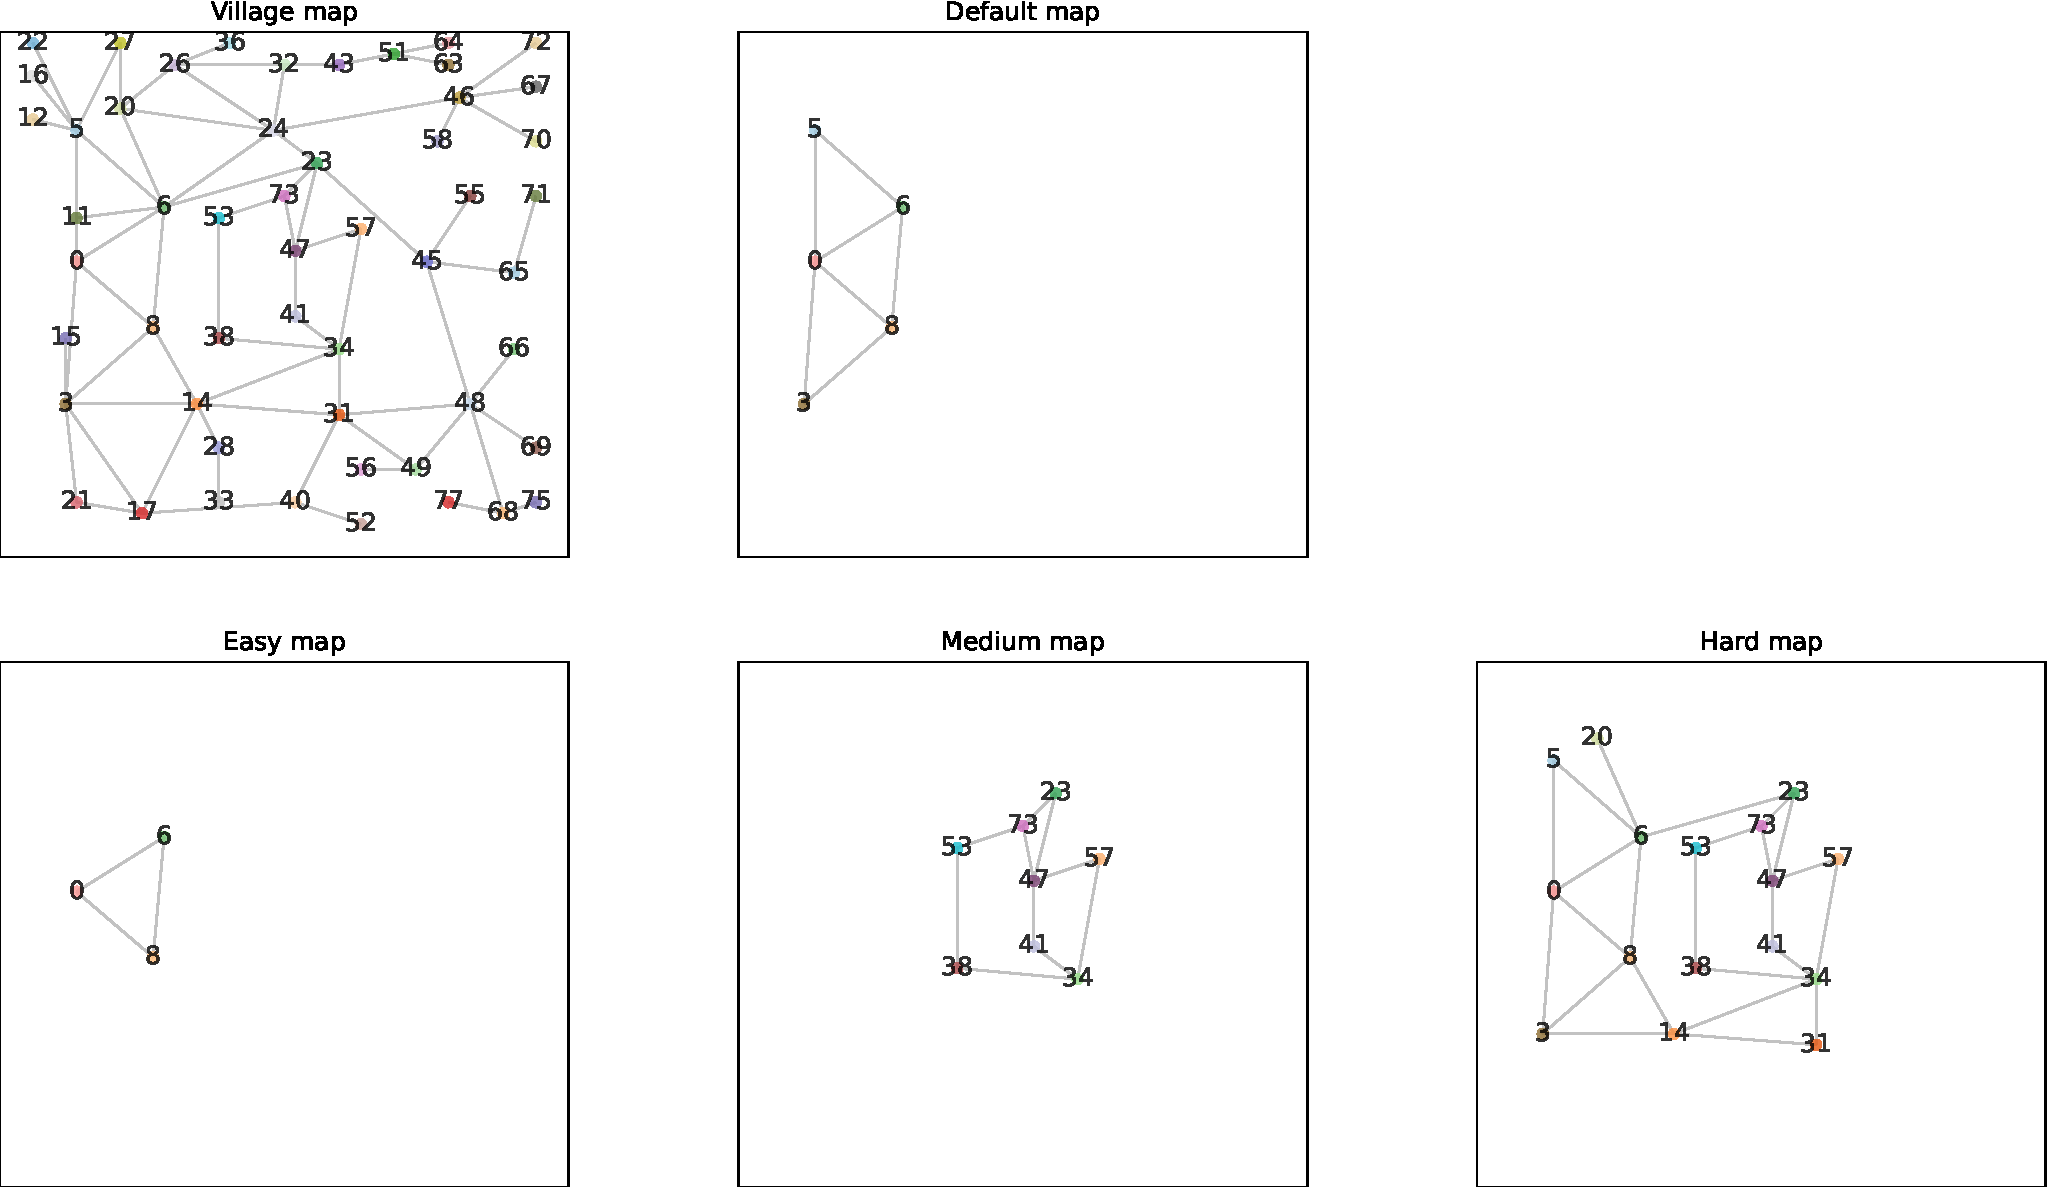
\includegraphics[width=0.68\linewidth,keepaspectratio]{figures/all_graphs.pdf}
  \caption{Use backup visuals when a question needs more detail than the main deck can carry.}
\end{figure}
\end{frame}

\end{document}
